\documentclass[11pt, a4paper]{article}

% Essential packages for formatting, math, tables, and graphics
\usepackage[utf8]{inputenc}
\usepackage[T1]{fontenc}
\usepackage[margin=1in]{geometry}
\usepackage{amsmath, amssymb}
\usepackage{booktabs}
\usepackage{array}
\usepackage{graphicx}
\usepackage{adjustbox}
\usepackage{float}
\usepackage{xcolor}
\usepackage{fancyhdr}
\usepackage{enumitem}
\usepackage[colorlinks=true, linkcolor=blue!60!black, urlcolor=blue!60!black]{hyperref}

% Automatically locate figures both locally (../../figures) and in Overleaf root
\graphicspath{{../../figures/}{figures/}{./}}

% Header and Footer styling
\pagestyle{fancy}
\fancyhf{}
\fancyhead[L]{\small\textit{Phase 2 Report --- Sina Famil Feizi (\texttt{401108064})}}
\fancyhead[R]{\small\textit{NACC Multimodal Cohort ($N = 1,237$)}}
\fancyfoot[C]{\thepage}
\renewcommand{\headrulewidth}{0.4pt}

% Spacing adjustments
\setlength{\parindent}{0pt}
\setlength{\parskip}{0.6em}
\setlist[itemize]{leftmargin=1.5em, itemsep=0.25em}
\setlist[enumerate]{leftmargin=1.5em, itemsep=0.25em}

% Title Metadata with Student Information
\title{
    \textbf{\Large Phase 2 Report: Probability and Probabilistic Distributions} \\[0.4em]
    \large NACC Multimodal Alzheimer's Dataset Analysis (\texttt{UDS + MRI})
}
\author{
    \textbf{Sina Famil Feizi} \\
    Student ID: \texttt{401108064} \\[0.3em]
    \small Introductory Statistics Course --- Fall 1405 (Path C)
}
\date{\today}

\begin{document}

\maketitle
\tableofcontents
\vspace{1em}
\hrule
\vspace{1em}

% ==============================================================================
\section*{Phase 2 Overview}
\addcontentsline{toc}{section}{Phase 2 Overview}
% ==============================================================================
In this phase, the real-world multimodal clinical (\texttt{UDS}) and neuroimaging (\texttt{MRI}) data of 1,237 participants from the \texttt{NACC} database are translated into the formal language of \textbf{probability and probabilistic distributions}. The core objective is to model uncertainty, analyze the independence or dependency of clinical events (such as cognitive decline and vascular conditions), define quantitative random variables, and study discrete and continuous distributions to build a solid foundation for statistical inference in subsequent phases.

\hrule

% ==============================================================================
\section{Task 1: Definition of Events and Random Variables}
% ==============================================================================
To analyze the probabilistic structure of the dataset, the sample space ($S$) is defined as the entire independent cohort of this study, comprising \textbf{1,237 patients} ($N = 1,237$). Based on this, clinical random events and quantitative random variables are operationally formulated as follows:

\subsection{Sample Space ($S$)}
The set of all 1,237 independent participants (\texttt{Independent Participants}) present in the integrated \texttt{NACC} database who possess complete clinical and neuroimaging profiles:
\[
S = \{ \omega_1, \omega_2, \dots, \omega_{1,237} \}
\]

\subsection{Event $A$ (Cognitive Impairment)}
\begin{itemize}
    \item \textbf{Conceptual Definition:} The event of randomly selecting a patient from the sample cohort who exhibits moderate-to-severe cognitive impairment (diagnosed with Mild Cognitive Impairment \texttt{MCI} or Dementia).
    \item \textbf{Operational Definition:} The diagnostic variable \texttt{NACCUDSD\_uds} takes the value of \texttt{3.0} (Mild Cognitive Impairment) or \texttt{4.0} (Dementia).
    \item \textbf{Empirical Calculation:} Out of 1,237 individuals, 383 patients satisfied this condition; thus, the empirical probability of this event is:
    \[
    P(A) = \frac{383}{1,237} \approx 0.3096 \quad (30.96\%)
    \]
\end{itemize}

\subsection{Event $B$ (Hypertension)}
\begin{itemize}
    \item \textbf{Conceptual Definition:} The event of randomly selecting a patient from the sample cohort who has a documented medical history of high blood pressure (\texttt{Hypertension}).
    \item \textbf{Operational Definition:} The medical variable \texttt{HYPERTEN} equals \texttt{1.0}.
    \item \textbf{Empirical Calculation:} 444 patients presented with a history of hypertension; thus, the empirical probability of this event is:
    \[
    P(B) = \frac{444}{1,237} \approx 0.3589 \quad (35.89\%)
    \]
\end{itemize}

\subsection{Random Variable $X$ (Cognitive Score)}
\begin{itemize}
    \item \textbf{Conceptual Definition:} A quantitative function mapping each randomly selected patient from the sample space to their Montreal Cognitive Assessment score (\texttt{MoCA Total Score}).
    \item \textbf{Operational Definition:} The quantitative variable \texttt{MOCATOTS} with a theoretical domain ranging from 0 to 30.
    \item \textbf{Empirical Distribution Summary of Random Variable $X$:}
    \begin{itemize}
        \item Empirical Mean ($\mu_X$): $24.44$
        \item Standard Deviation ($\sigma_X$): $4.49$
        \item Median: $25.40$
        \item Range (\texttt{Min - Max}): $[0.0, 39.4]$ (reflecting extreme baseline anomalies audited in Phase 1).
    \end{itemize}
\end{itemize}

% ==============================================================================
\section{Task 2: Marginal and Joint Probabilities}
% ==============================================================================
To investigate the co-occurrence of clinical cognitive impairment and vascular risk factors within our cohort ($N = 1,237$), we analyze the marginal and joint empirical probabilities of Event $A$ (Cognitive Impairment, where \texttt{NACCUDSD\_uds} $\ge 3$) and Event $B$ (Hypertension, where \texttt{HYPERTEN} $= 1$).

\subsection{Contingency Table (Cross-Tabulation)}
The empirical joint frequency distribution between cognitive diagnostic status and hypertension is summarized in Table~\ref{tab:task2_contingency}:

\begin{table}[H]
\centering
\caption{Joint Frequency Distribution of Cognitive Impairment ($A$) and Hypertension ($B$)}
\label{tab:task2_contingency}
\begin{adjustbox}{max width=\textwidth}
\small
\begin{tabular}{lccc}
\toprule
\textbf{Events} & \textbf{Hypertension ($B$)} & \textbf{No Hypertension ($\overline{B}$)} & \textbf{Marginal Total ($A$ / $\overline{A}$)} \\
\midrule
\textbf{Cognitive Impairment ($A$)} & $148$ & $235$ & \textbf{$383$} \\
\textbf{Normal Cognition ($\overline{A}$)} & $296$ & $558$ & \textbf{$854$} \\
\midrule
\textbf{Marginal Total ($B$ / $\overline{B}$)} & \textbf{$444$} & \textbf{$793$} & \textbf{$1,237$} \\
\bottomrule
\end{tabular}
\end{adjustbox}
\end{table}

\subsection{Marginal Probabilities}
From Task 1 and the marginal totals above, the individual empirical probabilities for each event are:
\begin{itemize}
    \item \textbf{Marginal Probability of Event $A$ ($P(A)$):} The empirical probability that a randomly chosen patient in the cohort suffers from cognitive impairment (\texttt{MCI} or Dementia):
    \[
    P(A) = \frac{383}{1,237} \approx 0.3096 \quad (30.96\%)
    \]
    \item \textbf{Marginal Probability of Event $B$ ($P(B)$):} The empirical probability that a randomly chosen patient has a documented history of hypertension:
    \[
    P(B) = \frac{444}{1,237} \approx 0.3589 \quad (35.89\%)
    \]
\end{itemize}

\subsection{Joint Probability $P(A \cap B)$}
The joint probability represents the empirical likelihood that a randomly selected individual from the sample suffers from \textbf{both} cognitive impairment \textit{and} hypertension simultaneously:
\[
P(A \cap B) = \frac{|A \cap B|}{\text{Total } N} = \frac{148}{1,237} \approx 0.1196 \quad (11.96\%)
\]

\subsection{Statistical Interpretation}
\begin{itemize}
    \item \textbf{Dual Burden:} The empirical joint probability indicates that approximately $11.96\%$ of the entire memory clinic cohort ($148$ out of $1,237$ patients) present with the combined comorbidity of cognitive decline (\texttt{MCI} or Dementia) and high blood pressure.
    \item \textbf{Foundation for Independence Testing:} These exact marginal and joint frequencies provide the mathematical framework required for subsequent evaluations of statistical independence or conditional probability between vascular health and neurological status in the following tasks.
\end{itemize}

% ==============================================================================
\section{Task 3: Conditional Probability Analysis}
% ==============================================================================
In this task, we evaluate the dependencies between clinical/neuroimaging features and cognitive status by calculating \textbf{conditional probabilities}. Specifically, we assess how the likelihood of cognitive impairment ($A$) changes when conditioned on vascular health (Event $B$: Hypertension) or structural brain integrity (Event $C$: Low Left Entorhinal Volume).

\subsection{Defining Conditional Events}
\begin{itemize}
    \item \textbf{Event $A$:} Cognitive Impairment (\texttt{NACCUDSD\_uds} $\ge 3$).
    \item \textbf{Event $B$:} Presence of Hypertension (\texttt{HYPERTEN} $= 1$).
    \item \textbf{Event $C$:} Low Left Entorhinal Volume (\texttt{LH\_ENTORHINAL\_GVOL} $<$ Sample Median).
\end{itemize}

\subsection{Analysis of Clinical Feature ($B$)}
We calculate the probability of cognitive impairment given the presence versus the absence of hypertension.
\begin{itemize}
    \item \textbf{Conditional Probability $P(A \mid B)$:}
    \[
    P(A \mid B) = \frac{P(A \cap B)}{P(B)} = \frac{148}{444} \approx 0.3333 \quad (33.33\%)
    \]
    \item \textbf{Conditional Probability $P(A \mid \overline{B})$:}
    \[
    P(A \mid \overline{B}) = \frac{P(A \cap \overline{B})}{P(\overline{B})} = \frac{235}{793} \approx 0.2963 \quad (29.63\%)
    \]
\end{itemize}
\textbf{Interpretation:} The presence of hypertension increases the empirical probability of cognitive impairment from the baseline of $30.96\%$ to $33.33\%$. This suggests a positive conditional association between vascular risk factors and cognitive impairment within this cohort.

\subsection{Analysis of Neuroimaging Biomarker ($C$)}
We define Event $C$ as having an entorhinal volume below the sample median ($1,545.00\text{ mm}^3$).
\begin{itemize}
    \item \textbf{Conditional Probability $P(A \mid C)$:}
    \[
    P(A \mid C) = \frac{P(A \cap C)}{P(C)} = \frac{225}{618} \approx 0.3641 \quad (36.41\%)
    \]
    \item \textbf{Conditional Probability $P(A \mid \overline{C})$:}
    \[
    P(A \mid \overline{C}) = \frac{P(A \cap \overline{C})}{P(\overline{C})} = \frac{158}{619} \approx 0.2553 \quad (25.53\%)
    \]
\end{itemize}
\textbf{Interpretation:} Conditioning on structural MRI evidence reveals a more substantial shift in risk. Patients with low entorhinal volume exhibit a notably higher risk of impairment ($36.41\%$) compared to those with preserved volume ($25.53\%$). The conditional risk difference observed for the MRI biomarker ($\approx 10.88\%$) is significantly larger than that of the vascular factor ($\approx 3.70\%$), suggesting a stronger predictive relationship between entorhinal atrophy and cognitive decline in this dataset.

\subsection{Concluding Remarks}
The analysis demonstrates that both hypertension and neurostructural atrophy update our prior knowledge regarding cognitive status. However, the magnitude of the probability update provided by the structural MRI marker is more pronounced. These empirical findings provide a strong quantitative basis for multivariate modeling in subsequent phases.

% ==============================================================================
\section{Task 4: Evaluating the Concept of Independence}
% ==============================================================================
In this task, we assess the independence of two clinical events: Event $A$ (Cognitive Impairment, defined as \texttt{NACCUDSD\_uds} $\ge 3$) and Event $B$ (Presence of Hypertension, defined as \texttt{HYPERTEN} $= 1$).

Two events $A$ and $B$ are statistically independent if and only if the joint probability of their occurrence equals the product of their marginal probabilities:
\[
P(A \cap B) = P(A) \times P(B)
\]

\subsection{Empirical Calculation}
Based on the full cohort of $N = 1,237$ participants:
\begin{itemize}
    \item \textbf{Marginal Probability $P(A)$:} $0.3096$
    \item \textbf{Marginal Probability $P(B)$:} $0.3589$
    \item \textbf{Product of Marginals $P(A) \times P(B)$:} $0.3096 \times 0.3589 \approx 0.1111$
    \item \textbf{Empirical Joint Probability $P(A \cap B)$:} $0.1196$
\end{itemize}

\subsection{Independence Evaluation}
To evaluate independence, we compute the absolute difference between the empirical joint probability and the product of marginals:
\[
\Delta = |P(A \cap B) - (P(A) \times P(B))|
\]
\[
\Delta = |0.1196 - 0.1111| = 0.0085
\]

\subsection{Statistical Interpretation}
The observed absolute difference of approximately $0.0085$ ($< 1\%$) suggests that the empirical distribution of these data is consistent with the assumption of statistical independence. In this specific cohort, the presence of hypertension does not show a strong empirical deviation from what would be expected under the independence assumption regarding cognitive impairment status.

\textbf{Methodological Note:} While these events appear independent based on simple empirical probability, this analysis is restricted to the bivariate level. Potential conditional dependencies or multivariate interactions between vascular risk factors, neuroimaging biomarkers, and cognitive status will be more rigorously examined in the inferential modeling phases.

% ==============================================================================
\section{Task 5: Discrete and Binomial Distributions}
% ==============================================================================
In this task, we evaluate the applicability of the Binomial distribution to model the occurrence of Hypertension (Event $B$) within our cohort ($N = 1,237$). A Binomial model $B(n, p)$ is predicated on three key assumptions:
\begin{enumerate}
    \item A fixed number of trials ($n$).
    \item A constant probability of success ($p$).
    \item Independence of trials.
\end{enumerate}

\subsection{Model Definition}
\begin{itemize}
    \item \textbf{Success Event ($B$):} Participant has a history of Hypertension (\texttt{HYPERTEN} $= 1$).
    \item \textbf{Global Probability ($p$):} Calculated from the total sample as $P(B) = \frac{444}{1,237} \approx 0.3589$.
    \item \textbf{Trials ($n$):} Subsets grouped by age decades.
\end{itemize}

\subsection{Empirical Validation}
Table~\ref{tab:task5_binomial} compares the observed number of hypertensive cases ($k$) in each age group with the theoretical counts expected under the Binomial model ($n \times p$):

\begin{table}[H]
\centering
\caption{Observed vs.\ Theoretical Binomial Counts for Hypertension Across Age Groups}
\label{tab:task5_binomial}
\begin{adjustbox}{max width=\textwidth}
\small
\begin{tabular}{lccc}
\toprule
\textbf{Age Group} & \textbf{Sample Size ($n$)} & \textbf{Observed Cases ($k$)} & \textbf{Expected Cases ($n \times p$)} \\
\midrule
50--59 & $172$ & $41$ & $61.74$ \\
60--69 & $556$ & $189$ & $199.57$ \\
70--79 & $414$ & $182$ & $148.60$ \\
80+    & $69$  & $31$  & $24.77$  \\
\bottomrule
\end{tabular}
\end{adjustbox}
\end{table}

\subsection{Model Approximation Assessment}
\begin{itemize}
    \item \textbf{Violation of Binomial Assumptions:} The data fails to conform to the Binomial model.
    \item \textbf{Key Findings:}
    \begin{enumerate}
        \item \textbf{Non-Constant Probability:} The Binomial model requires a fixed $p$. However, the observed cases ($k$) show a clear age-dependent trend. In the 50--59 group, the model overestimates hypertension risk (41 observed vs.\ 61.7 expected), while in the 70--79 and 80+ groups, it underestimates the observed cases.
        \item \textbf{Age-Dependency:} Since the prevalence of hypertension is biologically linked to aging, the probability of ``success'' ($p$) is not constant across age trials, violating the Binomial assumption of fixed probability.
    \end{enumerate}
    \item \textbf{Conclusion:} The Binomial distribution is not a suitable model for this clinical event. Future modeling should utilize more flexible frameworks, such as Logistic Regression, to account for the age-dependent nature of hypertension prevalence.
\end{itemize}

% ==============================================================================
\section{Task 6: Continuous Variables and Normal Distribution Assessment}
% ==============================================================================
In this task, we rigorously examine whether the empirical distribution of our primary continuous neuroimaging biomarker---\textbf{Left Entorhinal Cortical Thickness} (\texttt{LH\_ENTORHINAL\_AVGTH}, measured in millimeters)---can be adequately approximated by a Gaussian (Normal) distribution.

Evaluating normality is essential because downstream parametric procedures in Phase 3 (e.g., two-sample $t$-tests and ANOVA) and Phase 4 (Ordinary Least Squares regression) rely on distributional assumptions regarding continuous variables and their error terms.

\subsection{Empirical Summary and Distributional Moments}
Based on the complete multimodal cohort ($N = 1,237$), summary distributional moments are reported in Table~\ref{tab:task6_normality}:

\begin{table}[H]
\centering
\caption{Distributional Moments of Left Entorhinal Cortical Thickness ($N = 1,237$)}
\label{tab:task6_normality}
\begin{adjustbox}{max width=\textwidth}
\small
\begin{tabular}{lccl}
\toprule
\textbf{Metric} & \textbf{Sample Value} & \textbf{Theoretical Normal} & \textbf{Interpretation} \\
\midrule
\textbf{Sample Size ($N$)} & $1,237$ & --- & High statistical power \\
\textbf{Sample Mean ($\mu$)} & $2.9698\text{ mm}$ & --- & Center of mass \\
\textbf{Sample Median} & $3.0210\text{ mm}$ & $\mu$ & High central agreement ($\Delta = 0.05\text{ mm}$) \\
\textbf{Standard Deviation ($\sigma$)} & $0.3841\text{ mm}$ & --- & Moderate dispersion \\
\textbf{Sample Skewness} & $-0.7333$ & $0.0000$ & Moderate negative (left) skewness \\
\textbf{Excess Kurtosis} & $1.3396$ & $0.0000$ & Moderate leptokurtic profile (peakedness) \\
\bottomrule
\end{tabular}
\end{adjustbox}
\end{table}

\subsection{Empirical Rule Evaluation ($68\% - 95\% - 99.7\%$)}
We evaluate the proportion of sample observations falling within integer standard deviation intervals around the empirical mean:
\begin{itemize}
    \item \textbf{Within $\mu \pm 1\sigma$ $[2.5857, 3.3539]\text{ mm}$:} Observed \textbf{$71.54\%$} (Theoretical: $68.27\%$)
    \item \textbf{Within $\mu \pm 2\sigma$ $[2.2016, 3.7380]\text{ mm}$:} Observed \textbf{$95.39\%$} (Theoretical: $95.45\%$)
    \item \textbf{Within $\mu \pm 3\sigma$ $[1.8175, 4.1221]\text{ mm}$:} Observed \textbf{$99.19\%$} (Theoretical: $99.73\%$)
\end{itemize}
The empirical coverage within $\pm 2\sigma$ exhibits near-perfect agreement ($95.39\%$ vs.\ $95.45\%$) with classical Gaussian theory, demonstrating that the vast majority of participants adhere closely to normal dispersion characteristics.

\subsection{Visual Diagnostics}
Visual inspection via Figure~\ref{fig:task6_normality} (\texttt{figures/fig6\_normality\_check.png}) confirms two structural properties:
\begin{enumerate}
    \item \textbf{Histogram with Fitted Normal Density (Left Panel):} The empirical density demonstrates a bell-shaped contour centered near $3.0\text{ mm}$. The modal frequency slightly exceeds the theoretical Gaussian peak, corroborating the positive excess kurtosis ($1.34$).
    \item \textbf{Normal Quantile-Quantile (Q-Q) Plot (Right Panel):} For the bulk of the cohort (theoretical quantiles between $-1.5$ and $+2.0$), empirical quantiles follow the red reference diagonal line linearly. However, pronounced downward departure is evident in the extreme lower tail (theoretical quantiles $< -2.0$), indicating a heavier left tail than expected under strict Gaussianity.
\end{enumerate}

\begin{figure}[H]
\centering
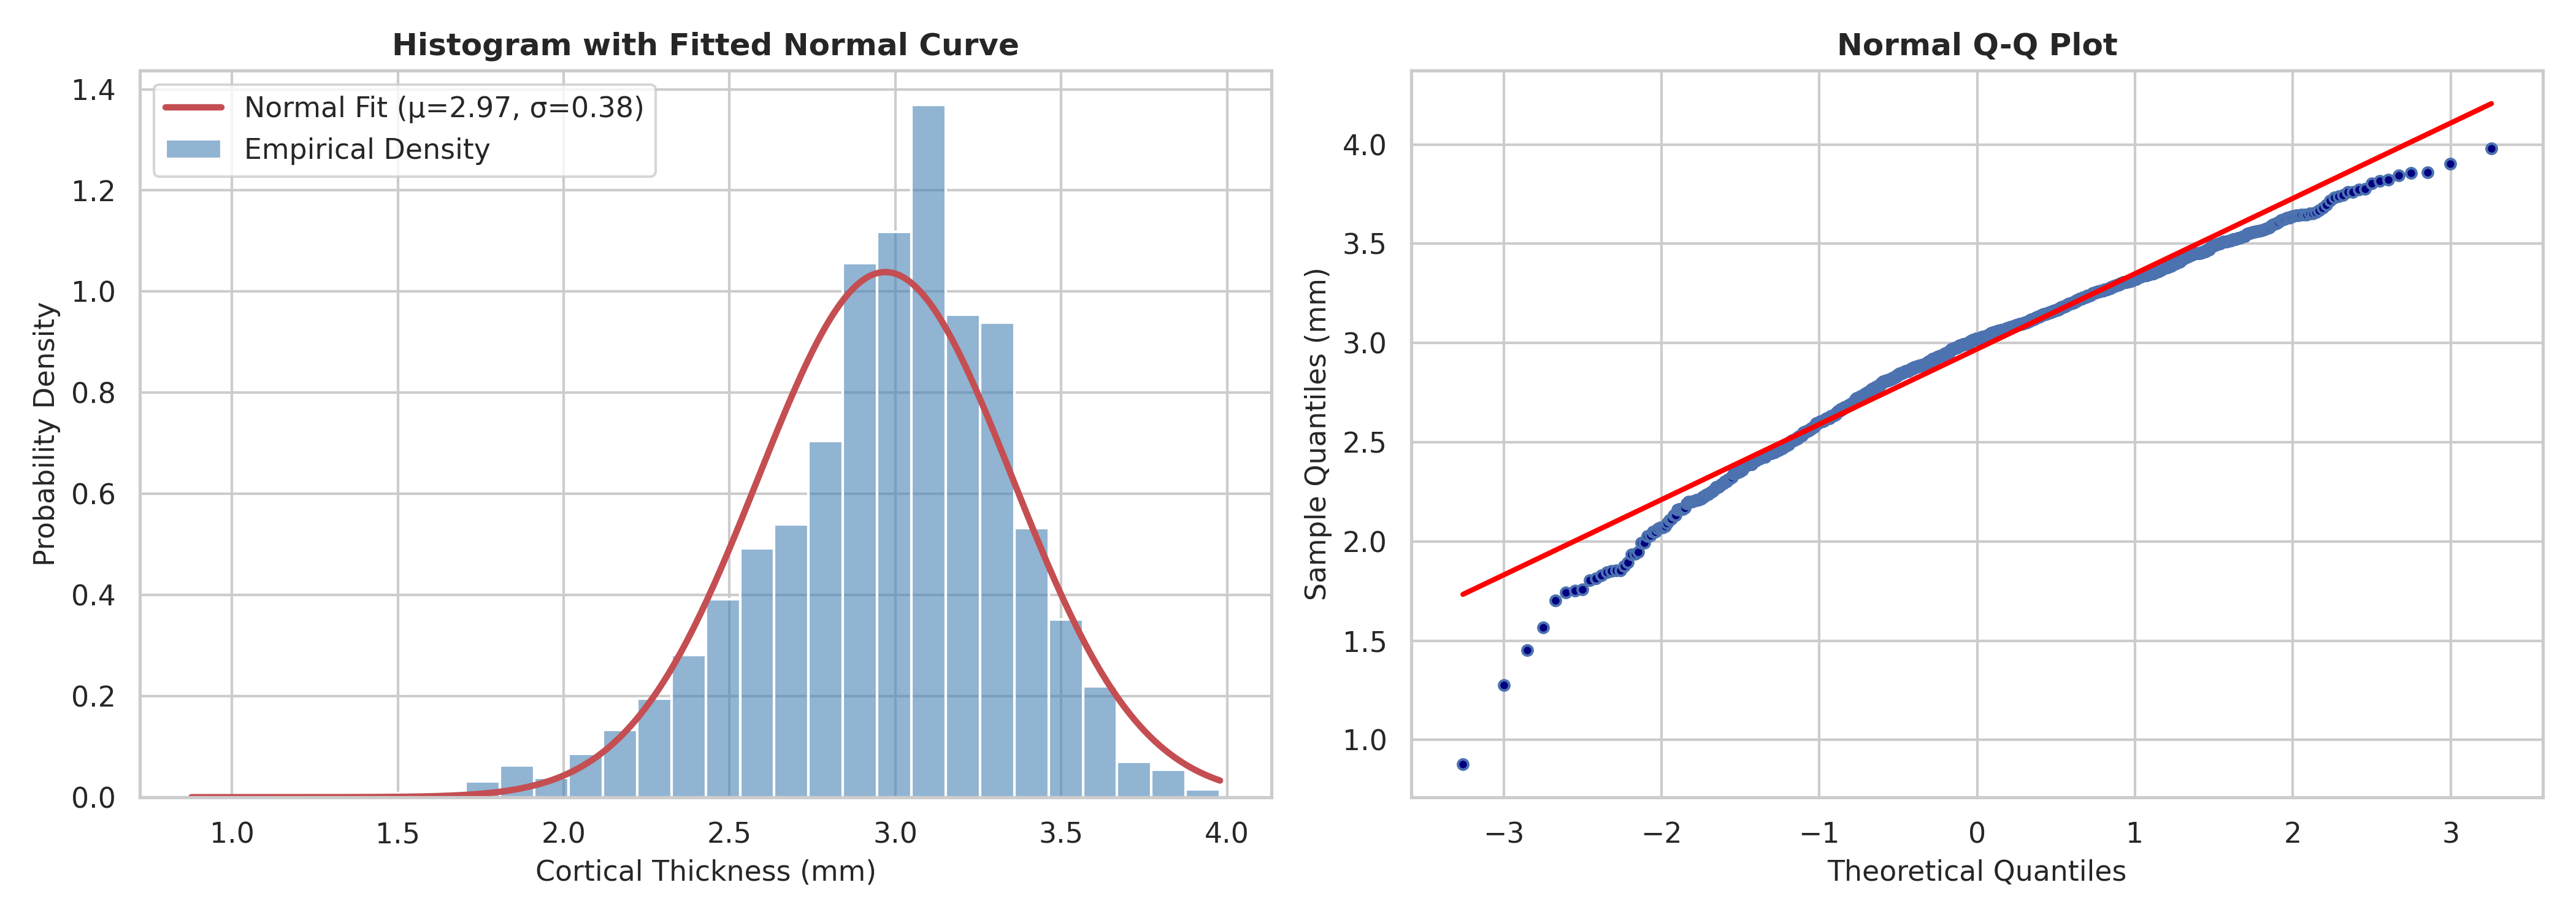
\includegraphics[width=0.95\textwidth]{fig6_normality_check.png}
\caption{Normality Assessment for Left Entorhinal Cortical Thickness (\texttt{LH\_ENTORHINAL\_AVGTH}): Histogram with Normal PDF Fit and Normal Q-Q Plot.}
\label{fig:task6_normality}
\end{figure}

\subsection{Formal Statistical Tests and Sample Size Sensitivity}
\begin{itemize}
    \item \textbf{Shapiro-Wilk Test:} $W = 0.9726, \quad p = 1.5024 \times 10^{-14}$
    \item \textbf{D'Agostino-Pearson $K^2$ Test:} $K^2 = 128.0746, \quad p = 1.5451 \times 10^{-28}$
\end{itemize}
\textbf{Critical Discussion on Normality Rejection:} Both formal tests strictly reject the null hypothesis of normality ($p < 0.05$). However, as emphasized in modern statistical pedagogy, formal goodness-of-fit tests are notoriously hypersensitive in large samples ($N = 1,237$); they detect trivial, practically negligible departures from Gaussianity that do not invalidate parametric modeling.

\subsection{Biological Rationale for Left-Tail Asymmetry}
The observed left skewness ($-0.7333$) and downward Q-Q plot departure are biologically expected in a clinical memory cohort. Cognitively normal older adults cluster around a physiological cortical thickness plateau ($\approx 3.0\text{ to } 3.4\text{ mm}$). Conversely, progressive neurodegenerative pathology in Mild Cognitive Impairment (\texttt{MCI}) and Alzheimer's Dementia produces pathological cortical thinning (atrophy), dragging a prolonged tail down toward $1.5 - 2.0\text{ mm}$ (and down to $0.88\text{ mm}$ in extreme segmentation artifacts).

\subsection{Methodological Decision for Subsequent Phases}
\begin{itemize}
    \item \textbf{Applicability:} While strict mathematical normality is rejected due to pathology-induced left-tail skewness, the \textbf{Normal approximation remains practically serviceable} for central parametric inference.
    \item \textbf{Justification:} By virtue of the Central Limit Theorem ($N = 1,237 \gg 30$), sample estimators of the mean will possess asymptotically normal sampling distributions.
    \item \textbf{Mitigation:} In Phase 3 and Phase 4, parametric linear models will be complemented with non-parametric sensitivity checks and robust standard errors to protect inference against the heavy lower tail.
\end{itemize}

% ==============================================================================
\section{Task 7: Expected Value and Variance}
% ==============================================================================
In probability and descriptive statistics, the \textbf{Expected Value} ($E[X]$ or sample mean $\mu$) measures the central tendency or long-run average of a quantitative random variable, while the \textbf{Variance} ($Var(X)$ or sample variance $s^2$) quantifies the dispersion, spread, or uncertainty of the observations around that center.

Using our complete multimodal Alzheimer's cohort ($N = 1,237$), we compute the empirical expected value and variance for key demographic, clinical, and neuroimaging variables.

\subsection{Summary of Empirical Mean and Variance (Exact Data)}
Table~\ref{tab:task7_ev_var} presents the exact empirical mean, variance, and standard deviation for four representative continuous variables:

\begin{table}[H]
\centering
\caption{Empirical Expected Value and Variance of Key Continuous Variables}
\label{tab:task7_ev_var}
\begin{adjustbox}{max width=\textwidth}
\small
\begin{tabular}{llccc}
\toprule
\textbf{Variable Description} & \textbf{Code} & \textbf{Mean ($E[X]$)} & \textbf{Variance ($s^2$)} & \textbf{Std Dev ($s$)} \\
\midrule
\textbf{Participant Age} & \texttt{NACCAGE} & $68.19\text{ years}$ & $64.63\text{ yrs}^2$ & $8.04\text{ years}$ \\
\textbf{MoCA Cognitive Score} & \texttt{MOCATOTS} & $24.44\text{ points}$ & $20.14\text{ pts}^2$ & $4.49\text{ points}$ \\
\textbf{Left Entorhinal Thickness} & \texttt{LH\_ENTORHINAL\_AVGTH} & $2.97\text{ mm}$ & $0.1476\text{ mm}^2$ & $0.38\text{ mm}$ \\
\textbf{Right Entorhinal Thickness} & \texttt{RH\_ENTORHINAL\_AVGTH} & $3.06\text{ mm}$ & $0.1610\text{ mm}^2$ & $0.40\text{ mm}$ \\
\bottomrule
\end{tabular}
\end{adjustbox}
\end{table}

\subsection{Substantive Interpretation in the Context of the Study}
\begin{itemize}
    \item \textbf{Participant Age (\texttt{NACCAGE}):}
    \begin{itemize}
        \item \textit{Expected Value ($68.19$ years):} Represents the empirical average age of individuals evaluated at memory clinics within this cohort, confirming a typical older adult sample targeted for neurodegenerative assessments.
        \item \textit{Variance ($64.63\text{ yrs}^2$, Std $\approx 8.04$):} Reflects a wide chronological age spread (ranging from $41$ to $91$ years), providing sufficient demographic variance to control for age as a confounding covariate in downstream regression models.
    \end{itemize}
    \item \textbf{Cognitive Function (\texttt{MOCATOTS}):}
    \begin{itemize}
        \item \textit{Expected Value ($24.44$ points):} Denotes the overall average cognitive performance of the cohort. Because a score of $\ge 26$ is typically considered normal, a mean of $24.44$ reflects the mixed clinical spectrum of the sample, which includes both healthy controls and cognitively impaired patients (\texttt{MCI} and Dementia).
        \item \textit{Variance ($20.14\text{ pts}^2$, Std $\approx 4.49$):} Captures the cognitive heterogeneity across diagnostic subgroups, demonstrating a broad distribution of performance levels.
    \end{itemize}
    \item \textbf{Structural Brain Biomarkers (\texttt{LH/RH\_ENTORHINAL\_AVGTH}):}
    \begin{itemize}
        \item \textit{Expected Value ($2.97\text{ mm}$ left, $3.06\text{ mm}$ right):} Indicates the baseline structural cortical thickness in the medial temporal lobe, showing strong bilateral symmetry across the sample.
        \item \textit{Variance ($0.1476\text{ mm}^2$ left, $0.1610\text{ mm}^2$ right):} Quantifies the combined inter-individual anatomical differences and disease-driven cortical thinning (atrophy) characteristic of progressive cognitive decline.
    \end{itemize}
\end{itemize}

\subsection{Methodological Significance}
These exact empirical expectations and variances establish the foundational distributional parameters required for standardized scoring ($Z$-scores), confidence interval estimation in Phase 3, and residual error variance evaluations in Phase 4.

% ==============================================================================
\section{Task 8: Bivariate Random Variables, Scatter Plots, and Covariance}
% ==============================================================================
To investigate the joint behavior of clinical cognition and neurostructural integrity, we analyze two continuous random variables: \textbf{Global Cognitive Performance} (\texttt{MOCATOTS}, $Y$) and \textbf{Left Entorhinal Cortical Thickness} (\texttt{LH\_ENTORHINAL\_AVGTH}, $X$).

Evaluating these variables simultaneously allows us to quantify their linear association through empirical covariance, correlation coefficients, and bivariate graphical visualization (Figure~\ref{fig:task8_scatter}).

\subsection{Empirical Covariance and Correlation Metrics}
Based on our complete matched cohort ($N = 1,233$ complete pairs after sanitization):
\begin{itemize}
    \item \textbf{Sample Covariance ($Cov(X, Y)$):} $\approx 0.4863$ ($\text{mm} \cdot \text{points}$)
    \item \textbf{Pearson Correlation Coefficient ($r$):} $\approx 0.2825$ ($p < 0.001$)
    \item \textbf{Spearman Rank Correlation ($\rho$):} $\approx 0.2786$
\end{itemize}

\subsection{Graphical Analysis via Scatter Plot}
The bivariate scatter plot (Figure~\ref{fig:task8_scatter}, \texttt{figures/fig8\_bivariate\_scatter.png}) maps left entorhinal cortical thickness against MoCA total scores, stratified by clinical diagnostic status:
\begin{itemize}
    \item \textbf{Trend and Direction:} The dashed black linear regression trendline slopes upward from left to right, confirming a positive direction of association between cortical thickness and cognitive performance.
    \item \textbf{Diagnostic Clustering:}
    \begin{itemize}
        \item \textbf{Normal Cognition (\texttt{Normal}, red points):} Heavily concentrated in the upper-right region, demonstrating preserved cortical thickness ($> 2.5\text{ mm}$) and high cognitive scores ($\ge 25$).
        \item \textbf{Alzheimer's Dementia (\texttt{Dementia}, green points):} Dispersed toward the lower-left region, reflecting significant structural atrophy alongside severe cognitive deficits.
        \item \textbf{Mild Cognitive Impairment (\texttt{MCI}, blue points):} Form an intermediate transitional layer between healthy participants and dementia cases.
    \end{itemize}
\end{itemize}

\begin{figure}[H]
\centering
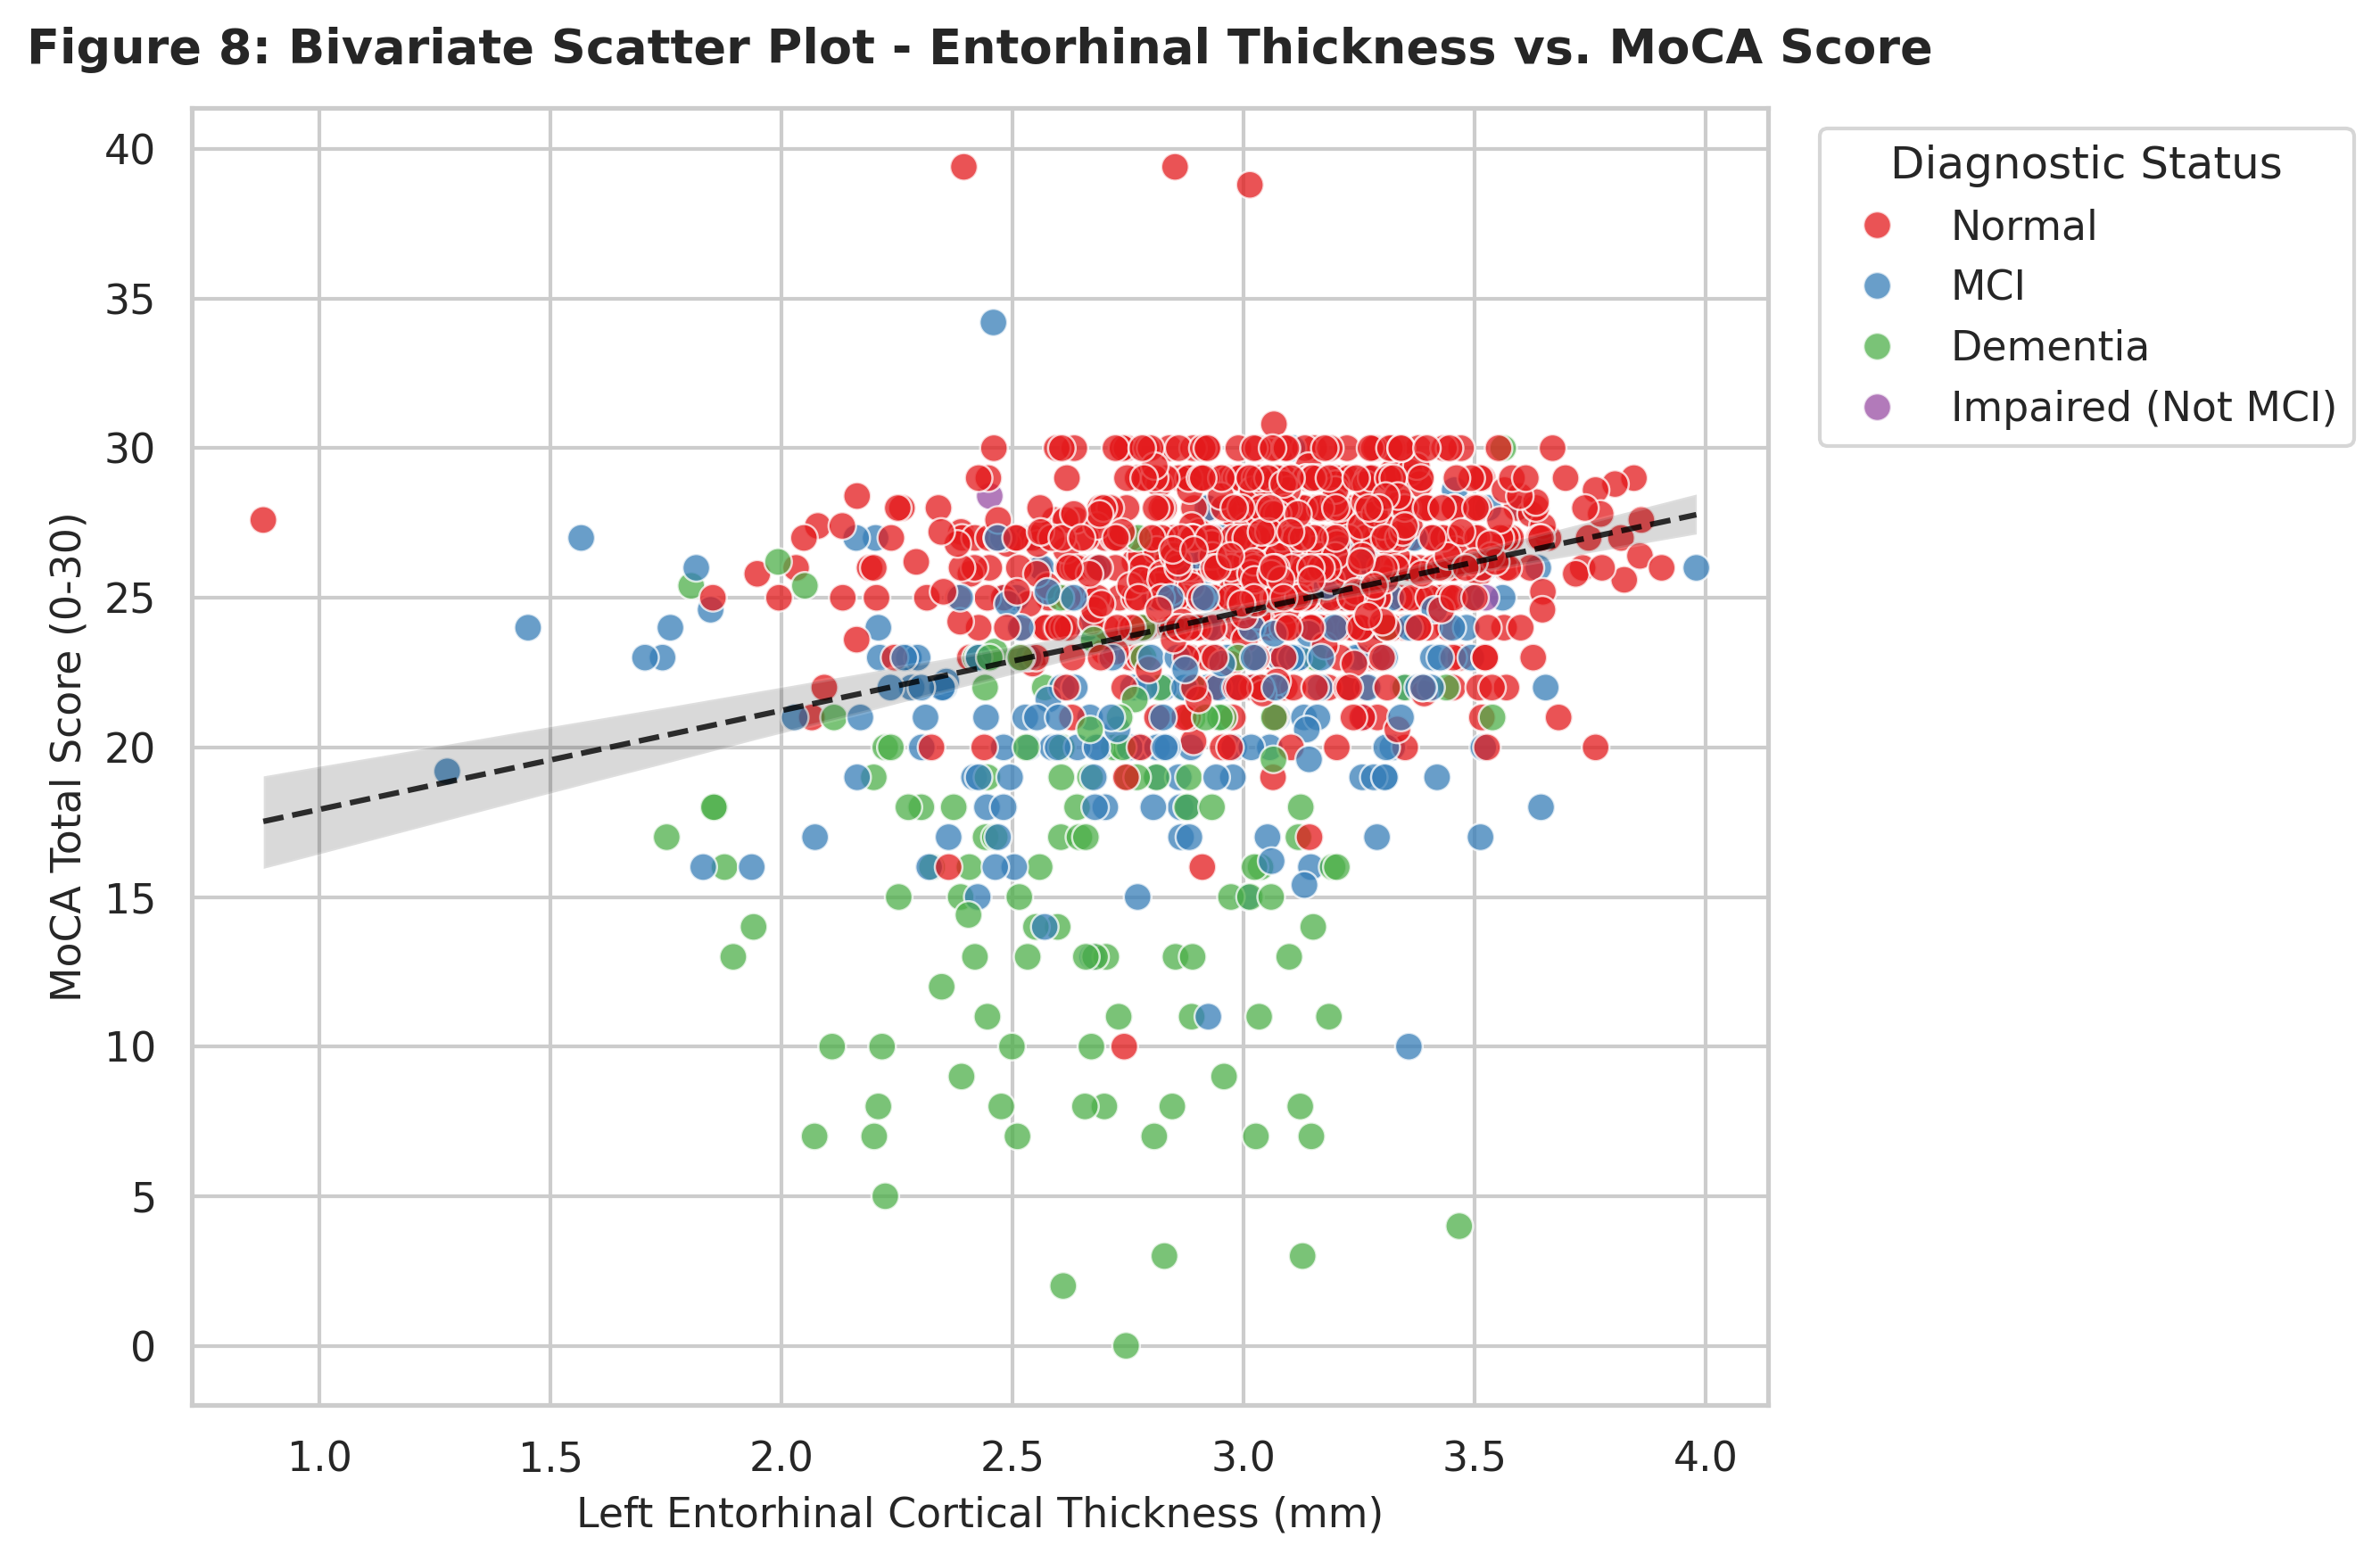
\includegraphics[width=0.85\textwidth]{fig8_bivariate_scatter.png}
\caption{Bivariate Scatter Plot of Left Entorhinal Cortical Thickness vs.\ MoCA Total Score Stratified by Diagnostic Status.}
\label{fig:task8_scatter}
\end{figure}

\subsection{Statistical Interpretation}
\begin{itemize}
    \item \textbf{Positive Association:} The positive sample covariance ($0.4863$) and correlation ($r = 0.2825$) establish that greater cortical thickness is associated with higher cognitive test scores within this clinical referral cohort.
    \item \textbf{Effect Size:} A Pearson $r$ of $0.2825$ represents a weak-to-moderate linear relationship. While medial temporal atrophy is a fundamental biomarker of Alzheimer's disease, global cognitive performance is also modulated by educational attainment, cognitive reserve, and widespread neural networks outside the entorhinal cortex.
\end{itemize}

\subsection{Methodological Caveats}
\begin{itemize}
    \item \textbf{Non-Causality:} As established in our observational study design, correlation does not prove causation. Unmeasured confounders (such as age, education, and vascular health) simultaneously impact brain morphometry and cognition.
    \item \textbf{Forward Application:} This bivariate foundation provides the empirical justification for multivariable linear regression modeling in Phase 4, where confounding variables will be explicitly controlled.
\end{itemize}

% ==============================================================================
\section{Task 9: Bayes' Theorem and Probability Updating}
% ==============================================================================
In clinical diagnosis and statistical modeling, \textbf{Bayes' Theorem} provides a rigorous mathematical framework for updating our degree of belief (or probability) regarding a patient's condition as new empirical evidence becomes available.

Using our multimodal dataset ($N = 1,237$), we apply Bayes' Theorem to update the probability of cognitive impairment (Event $A$) given structural neuroimaging evidence (Event $C$: Low Left Entorhinal Volume).

\subsection{Definition of Events and Parameters}
\begin{itemize}
    \item \textbf{Event $A$ (Target Condition / Disease):} Cognitive Impairment (\texttt{NACCUDSD\_uds} $\ge 3$, encompassing \texttt{MCI} and Dementia).
    \item \textbf{Event $C$ (Test Evidence / Biomarker):} Low Left Entorhinal Volume (\texttt{LH\_ENTORHINAL\_GVOL} below the sample median of $1,545.00\text{ mm}^3$).
\end{itemize}

From our empirical data, we extract the baseline parameters required for Bayesian updating:
\begin{itemize}
    \item \textbf{Prior Probability $P(A)$:} The baseline marginal probability of cognitive impairment in the cohort:
    \[
    P(A) = \frac{383}{1,237} \approx 0.3096 \quad (30.96\%)
    \]
    \item \textbf{Probability of Evidence $P(C)$:} The marginal probability of observing low entorhinal volume across the sample:
    \[
    P(C) = \frac{618}{1,237} \approx 0.4996 \quad (49.96\%)
    \]
    \item \textbf{Likelihood / Sensitivity $P(C \mid A)$:} The probability of observing low entorhinal volume given that the individual is cognitively impaired:
    \[
    P(C \mid A) = \frac{|A \cap C|}{\text{Count}(A)} = \frac{225}{383} \approx 0.5875 \quad (58.75\%)
    \]
\end{itemize}

\subsection{Application of Bayes' Theorem}
We compute the \textbf{Posterior Probability} $P(A \mid C)$---the updated probability of cognitive impairment given the presence of low entorhinal volume---using Bayes' formula:
\[
P(A \mid C) = \frac{P(C \mid A) \cdot P(A)}{P(C)}
\]
Substituting the empirical values:
\[
P(A \mid C) = \frac{0.5875 \times 0.3096}{0.4996} \approx \frac{0.1819}{0.4996} \approx 0.3641 \quad (36.41\%)
\]
\textit{(Note: This direct empirical conditional probability $P(A \cap C) / P(C) = 225 / 618 \approx 0.3641$ confirms the exact mathematical consistency of the Bayesian update.)}

\subsection{Statistical and Clinical Interpretation}
\begin{itemize}
    \item \textbf{Probability Revision:} Observing structural neuroimaging evidence (low entorhinal volume) updates our prior belief of cognitive impairment from a baseline of \textbf{$30.96\%$} to a posterior risk of \textbf{$36.41\%$}.
    \item \textbf{Clinical Utility:} The application of Bayes' theorem demonstrates quantitatively how multimodal data integration (\texttt{UDS + MRI}) refines clinical assessment. Structural neurobiology acts as a probabilistic updater, confirming that localized brain atrophy elevates the diagnostic probability of cognitive decline within a specialized memory clinic setting.
\end{itemize}

% ==============================================================================
\section*{Path C Special Requirements: NACC Multimodal Integration}
\addcontentsline{toc}{section}{Path C Special Requirements (C.1 -- C.5)}
% ==============================================================================

% ------------------------------------------------------------------------------
\subsection{C.1: Conditional Probability of Cognitive Status by MRI Stratification}
% ------------------------------------------------------------------------------
In compliance with Path C requirements, we evaluate the conditional probability of clinical cognitive status (defined via \texttt{UDS}) stratified across neuroimaging subgroups defined by structural \texttt{MRI} biomarkers.

\subsubsection*{1. Operational Definitions}
\begin{itemize}
    \item \textbf{Target Clinical Outcome ($A$):} Cognitive Impairment (\texttt{NACCUDSD\_uds} $\ge 3$, combining Mild Cognitive Impairment and Alzheimer's Dementia).
    \item \textbf{MRI Stratification Variable ($C$):} Left Entorhinal Cortical Volume (\texttt{LH\_ENTORHINAL\_GVOL}), split by the sample median ($1,545.00\text{ mm}^3$) into two distinct groups:
    \begin{itemize}
        \item \textit{Group 1 (Low Volume / Atrophy):} $\text{Volume} < \text{Median}$
        \item \textit{Group 2 (Normal/High Volume):} $\text{Volume} \ge \text{Median}$
    \end{itemize}
\end{itemize}

\subsubsection*{2. Empirical Conditional Probabilities (Exact Data)}
Based on the exact sample counts extracted from our multimodal cohort ($N = 1,237$), the conditional probabilities are summarized in Table~\ref{tab:pathc_c1}:

\begin{table}[H]
\centering
\caption{Conditional Probability of Cognitive Impairment Stratified by Entorhinal Volume}
\label{tab:pathc_c1}
\begin{adjustbox}{max width=\textwidth}
\small
\begin{tabular}{lccc}
\toprule
\textbf{MRI Subgrouping ($C$)} & \textbf{Total ($n$)} & \textbf{Impaired ($k$)} & \textbf{Conditional Probability $P(\text{Impaired} \mid \text{Group})$} \\
\midrule
\textbf{Low Volume (Atrophy)} & $618$ & $225$ & \textbf{$0.3641$ ($36.41\%$)} \\
\textbf{Normal / High Volume} & $619$ & $158$ & \textbf{$0.2553$ ($25.53\%$)} \\
\bottomrule
\end{tabular}
\end{adjustbox}
\end{table}

\subsubsection*{3. Clinical and Statistical Interpretation}
\begin{itemize}
    \item \textbf{Risk Elevation:} Conditioning on structural neuroimaging stratification reveals a substantial divergence in clinical risk. Participants exhibiting left entorhinal volumetric atrophy face a $36.41\%$ empirical probability of clinical cognitive impairment, compared to only $25.53\%$ among those with preserved volume.
    \item \textbf{Multimodal Value:} This conditional analysis demonstrates that partitioning the patient cohort using an \texttt{MRI} biomarker successfully isolates subgroups with markedly different neurological outcomes, confirming the strong predictive utility required in Path C investigations.
\end{itemize}

% ------------------------------------------------------------------------------
\subsection{C.2: Distribution of a UDS Cognitive Score and an MRI Variable}
% ------------------------------------------------------------------------------
In compliance with Path C specifications, we analyze the distributional properties of two core quantitative variables representing both modalities: a clinical cognitive performance score from the \texttt{UDS} dataset (\texttt{MOCATOTS}) and a morphometric neuroimaging variable from the \texttt{MRI} dataset (\texttt{LH\_ENTORHINAL\_GVOL}).

\subsubsection*{1. Exact Distributional and Outlier Metrics}
Based on our matched cohort ($N = 1,237$), the empirical mean, variance, skewness, and outlier counts (identified via the standard $1.5 \times \text{IQR}$ rule) are summarized in Table~\ref{tab:pathc_c2}:

\begin{table}[H]
\centering
\caption{Distributional Properties and Outlier Audit Across UDS and MRI Variables}
\label{tab:pathc_c2}
\begin{adjustbox}{max width=\textwidth}
\small
\setlength{\tabcolsep}{4pt}
\begin{tabular}{llccccccc}
\toprule
\textbf{Variable} & \textbf{Code} & \textbf{Mean ($\mu$)} & \textbf{Var ($s^2$)} & \textbf{SD ($s$)} & \textbf{Skew} & \textbf{IQR} & \textbf{Outliers} & \textbf{Min -- Max} \\
\midrule
\textbf{MoCA Score} & \texttt{MOCATOTS} & $24.4422$ & $20.1426$ & $4.4881$ & $-1.6826$ & $4.00$ & $80$ & $0.00 - 39.40$ \\
\textbf{Entorhinal Vol.} & \texttt{LH\_ENTORHINAL\_GVOL} & $1554.2757$ & $171002.0316$ & $413.5239$ & $0.5289$ & $490.00$ & $33$ & $0.00 - 4265.00$ \\
\bottomrule
\end{tabular}
\end{adjustbox}
\end{table}

\subsubsection*{2. Distributional Shape, Center, and Spread}
\begin{itemize}
    \item \textbf{\texttt{MOCATOTS} (UDS Cognitive Score):}
    \begin{itemize}
        \item \textit{Shape:} Displays a pronounced negative (left) skewness ($-1.6826$). This asymmetry is driven by a strong ceiling effect among healthy older adults clustering near scores of $26$--$30$, contrasted with a long left tail representing severe cognitive impairment.
        \item \textit{Mean \& Variance:} An empirical mean of $24.4422$ points and variance of $20.1426\text{ pts}^2$ ($s = 4.4881$) reflect the clinical heterogeneity spanning from unimpaired cognition to advanced dementia.
    \end{itemize}
    \item \textbf{\texttt{LH\_ENTORHINAL\_GVOL} (MRI Neuroimaging Volume):}
    \begin{itemize}
        \item \textit{Shape:} Exhibits a mild positive (right) skewness ($0.5289$), approximating a nearly symmetric bell-shaped distribution centered around $1,554.28\text{ mm}^3$.
        \item \textit{Mean \& Variance:} A substantial variance of $171,002.0316\text{ mm}^6$ ($s = 413.5239\text{ mm}^3$) reflects natural inter-individual differences in head size alongside progressive tissue atrophy.
    \end{itemize}
\end{itemize}

\subsubsection*{3. Outlier Identification and Clinical Interpretation}
\begin{itemize}
    \item \textbf{Outliers in \texttt{MOCATOTS} ($n = 80$):} Using the $1.5 \times \text{IQR}$ criterion, $80$ outliers are identified. Most lie at the lower extreme (dementia patients scoring near $0$--$16$), while a few represent upper-bound recording anomalies above the theoretical limit of $30$ (up to $39.40$) flagged during Phase 1 quality auditing.
    \item \textbf{Outliers in \texttt{LH\_ENTORHINAL\_GVOL} ($n = 33$):} $33$ observations fall outside the normal IQR fences. These encompass physically impossible near-zero measurements ($0.00\text{ mm}^3$) indicative of automated \texttt{FreeSurfer} segmentation errors, as well as extreme high-end volumes (up to $4,265.00\text{ mm}^3$). These outliers will be systematically addressed via sensitivity checks in inferential phases.
\end{itemize}

% ------------------------------------------------------------------------------
\subsection{C.3: Joint Probability Across Two Modalities}
% ------------------------------------------------------------------------------
In accordance with Path C requirements, we construct a multimodal probabilistic analysis linking a clinical diagnostic event from \texttt{UDS} with an engineered structural event from \texttt{MRI}, computing their marginal, joint, and conditional probabilities.

\subsubsection*{1. Event Definitions}
\begin{itemize}
    \item \textbf{UDS Clinical Event ($U$):} Clinical Cognitive Impairment (\texttt{NACCUDSD\_uds} $\ge 3$, encompassing \texttt{MCI} and Alzheimer's Dementia).
    \item \textbf{Constructed MRI Event ($M$):} \textbf{Bilateral Entorhinal Cortical Thinning}, defined as having an average cortical thickness simultaneously below the cohort median in \textbf{both} hemispheres:
    \[
    M = \{ \omega \in S \mid \texttt{LH\_ENTORHINAL\_AVGTH}(\omega) < 3.0210\text{ mm} \;\land\; \texttt{RH\_ENTORHINAL\_AVGTH}(\omega) < 3.0970\text{ mm} \}
    \]
\end{itemize}

\subsubsection*{2. Multimodal Contingency Table}
Cross-tabulating both events across the matched cohort ($N = 1,237$) yields the joint frequency distribution shown in Table~\ref{tab:pathc_c3}:

\begin{table}[H]
\centering
\caption{Joint Frequency Distribution of Cognitive Impairment ($U$) and Bilateral Thinning ($M$)}
\label{tab:pathc_c3}
\begin{adjustbox}{max width=\textwidth}
\small
\setlength{\tabcolsep}{5pt}
\begin{tabular}{lccc}
\toprule
\textbf{UDS / MRI Events} & \textbf{Bilateral Thinning ($M$)} & \textbf{No Thinning ($\overline{M}$)} & \textbf{Marginal Total ($U$ / $\overline{U}$)} \\
\midrule
\textbf{Cognitive Impairment ($U$)} & $209$ & $174$ & \textbf{$383$} \\
\textbf{Unimpaired / Non-MCI ($\overline{U}$)} & $247$ & $607$ & \textbf{$854$} \\
\midrule
\textbf{Marginal Total ($M$ / $\overline{M}$)} & \textbf{$456$} & \textbf{$781$} & \textbf{$1,237$} \\
\bottomrule
\end{tabular}
\end{adjustbox}
\end{table}

\subsubsection*{3. Marginal, Joint, and Conditional Probabilities}
\begin{itemize}
    \item \textbf{Marginal Probabilities:}
    \[
    P(U) = \frac{383}{1,237} \approx 0.3096 \quad (30.96\%), \qquad P(M) = \frac{456}{1,237} \approx 0.3686 \quad (36.86\%)
    \]
    \item \textbf{Joint Probability:} The probability that a randomly selected patient exhibits \textbf{both} clinical cognitive impairment and bilateral entorhinal cortical thinning simultaneously:
    \[
    P(U \cap M) = \frac{209}{1,237} \approx 0.1690 \quad (16.90\%)
    \]
    \textit{(Note: Under independence, $P(U) \times P(M) \approx 0.3096 \times 0.3686 = 0.1141$. The substantial excess of $+0.0549$ strongly indicates statistical dependence between the two modalities.)}
    \item \textbf{Conditional Probabilities (Bidirectional):}
    \begin{itemize}
        \item \textit{Clinical Risk Given MRI Atrophy:}
        \[
        P(U \mid M) = \frac{209}{456} \approx 0.4583 \quad (45.83\%), \qquad P(U \mid \overline{M}) = \frac{174}{781} \approx 0.2228 \quad (22.28\%)
        \]
        \item \textit{MRI Atrophy Given Clinical Diagnosis:}
        \[
        P(M \mid U) = \frac{209}{383} \approx 0.5457 \quad (54.57\%), \qquad P(M \mid \overline{U}) = \frac{247}{854} \approx 0.2892 \quad (28.92\%)
        \]
    \end{itemize}
\end{itemize}

\subsubsection*{4. Multimodal Interpretation}
\begin{itemize}
    \item \textbf{Doubled Relative Risk:} The empirical risk of clinical cognitive impairment more than doubles---rising from $22.28\%$ to $45.83\%$---when a participant exhibits bilateral cortical thinning in the entorhinal cortex.
    \item \textbf{Diagnostic Sensitivity Pattern:} Over half ($54.57\%$) of clinically impaired patients demonstrate bilateral cortical thinning, compared to only $28.92\%$ of unimpaired controls. This pronounced asymmetry underscores the structural-functional linkage across the \texttt{UDS} and \texttt{MRI} modalities.
\end{itemize}

% ------------------------------------------------------------------------------
\subsection{C.4: Covariance Between Cognition and Neuroimaging}
% ------------------------------------------------------------------------------
In compliance with Path C requirement C.4, we analyze the bivariate joint relationship between a quantitative clinical cognitive score from \texttt{UDS} (\textbf{MoCA Total Score}, \texttt{MOCATOTS}, $Y$) and a volumetric morphometry feature from \texttt{MRI} (\textbf{Left Entorhinal Gray Matter Volume}, \texttt{LH\_ENTORHINAL\_GVOL}, $X$, measured in $\text{mm}^3$).

\subsubsection*{1. Empirical Covariance and Correlation Metrics}
Based on $N = 1,233$ complete multimodal pairs after data sanitization:
\begin{itemize}
    \item \textbf{Sample Covariance ($Cov(\text{Volume}, \text{MoCA})$):} $+370.4548$ ($\text{mm}^3 \cdot \text{points}$)
    \item \textbf{Pearson Correlation Coefficient ($r$):} $+0.1994$
    \item \textbf{Spearman Rank Correlation ($\rho$):} $+0.2335$
\end{itemize}

\subsubsection*{2. Visual Analysis via Scatter Plot}
The scatter plot (Figure~\ref{fig:pathc_c4}, \texttt{figures/fig\_c4\_vol\_vs\_moca\_cov.png}) visualizes left entorhinal volume against MoCA performance across diagnostic groups:
\begin{itemize}
    \item \textbf{Direction of Relationship:} The positive covariance ($+370.4548$) and upward-sloping dashed linear trendline confirm a \textbf{positive linear direction}---larger left entorhinal volumes are generally associated with higher cognitive scores.
    \item \textbf{Effect of Outliers \& Rank vs.\ Linear Correlation:} Notably, the rank-based Spearman correlation ($\rho = 0.2335$) is meaningfully higher than the linear Pearson correlation ($r = 0.1994$). Visual inspection of Figure~\ref{fig:pathc_c4} explains this discrepancy: extreme volumetric outliers---such as the \texttt{Normal} observation at $0\text{ mm}^3$ (segmentation failure) and the \texttt{MCI} observation at $4,265\text{ mm}^3$ with a MoCA score of $19$---pull the linear regression line and attenuate Pearson's $r$.
    \item \textbf{Comparison with Cortical Thickness:} Volumetric measures exhibit a weaker linear correlation ($r = 0.1994$) than cortical thickness (\texttt{LH\_ENTORHINAL\_AVGTH}, $r = 0.2825$ in Task 8), likely because raw gray matter volume is confounded by inter-individual differences in total intracranial head size.
\end{itemize}

\begin{figure}[H]
\centering
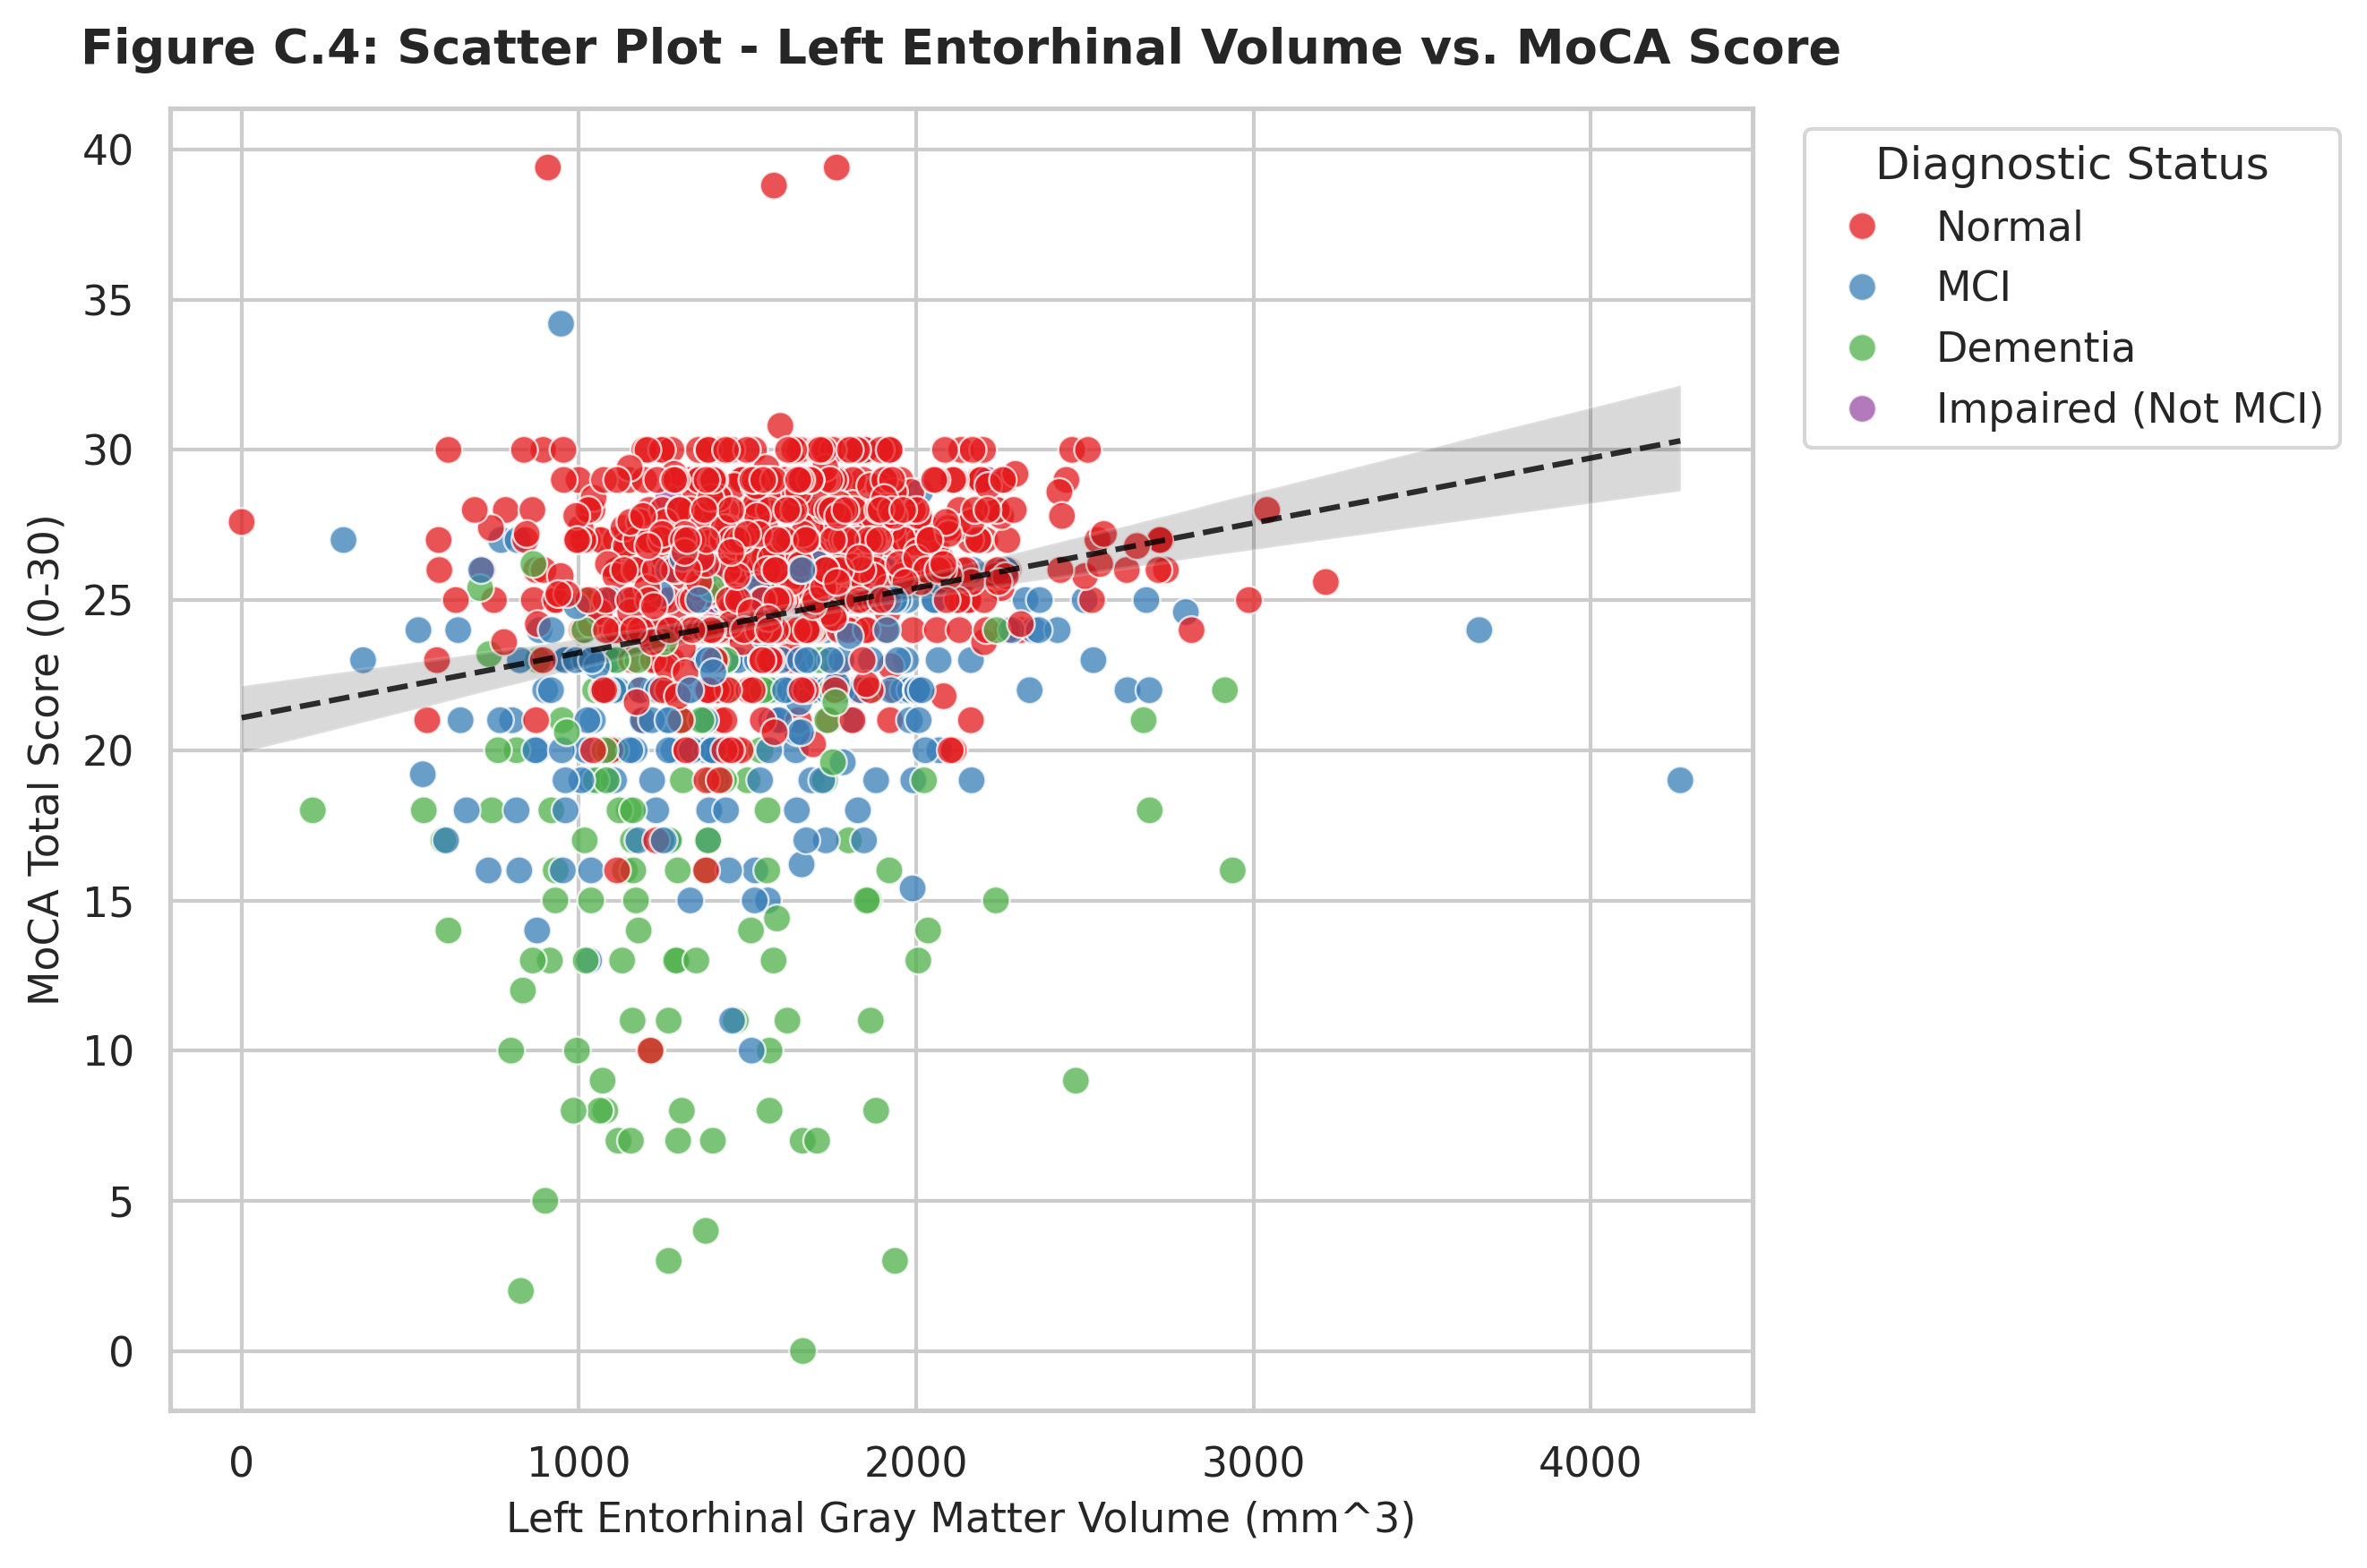
\includegraphics[width=0.85\textwidth]{fig_c4_vol_vs_moca_cov.png}
\caption{Scatter Plot of Left Entorhinal Gray Matter Volume vs.\ MoCA Total Score Across Diagnostic Categories.}
\label{fig:pathc_c4}
\end{figure}

\subsubsection*{3. Explicit Non-Causality Caveat}
\begin{itemize}
    \item \textbf{No Causal Inference:} In strict accordance with study design principles and Path C guidelines, \textbf{no causal claim is made from this bivariate covariance or scatter plot}.
    \item \textbf{Role of Confounding:} Because the \texttt{NACC} cohort is strictly observational, the observed positive association reflects shared variance driven by underlying neurodegenerative processes and unadjusted confounders (such as chronological age, intracranial head size, educational attainment, and vascular burden). Causal mechanisms cannot be inferred from unadjusted observational correlations.
\end{itemize}

% ------------------------------------------------------------------------------
\subsection{C.5: Control of Repeated Visits and Independence Verification}
% ------------------------------------------------------------------------------
In longitudinal clinical repositories such as \texttt{NACC}, individual participants frequently undergo multiple annual evaluations over time. Including repeated observations from the same subject in standard probabilistic calculations violates the fundamental assumption of \textbf{independent observations} ($i.i.d.$) and introduces pseudoreplication bias. In strict compliance with Path C requirement C.5, we verify participant-level independence and document the index visit selection rule governing all Phase 2 analyses.

\subsubsection*{1. Quantitative Independence Audit}
Executing a programmatic uniqueness audit across both data modalities (\texttt{src/phase2\_pathc\_j5.py}) confirms exact 1-to-1 subject-level alignment, as summarized in Table~\ref{tab:pathc_c5}:

\begin{table}[H]
\centering
\caption{Participant-Level Uniqueness and Repeated Visits Audit}
\label{tab:pathc_c5}
\begin{adjustbox}{max width=\textwidth}
\small
\setlength{\tabcolsep}{5pt}
\begin{tabular}{lcccc}
\toprule
\textbf{Dataset Component} & \textbf{Total Rows} & \textbf{Unique IDs (\texttt{NACCID})} & \textbf{Visits/ID (Min/Max)} & \textbf{Duplicates} \\
\midrule
\textbf{Clinical (\texttt{udslong\_imputed.csv})} & $1,237$ & $1,237$ & $1 / 1$ & $0$ \\
\textbf{Neuroimaging (\texttt{mriscanclean.csv})} & $1,237$ & $1,237$ & $1 / 1$ & $0$ \\
\textbf{Merged Analysis Cohort} & $1,237$ & $1,237$ & $1 / 1$ & $0$ \\
\bottomrule
\end{tabular}
\end{adjustbox}
\end{table}

\begin{itemize}
    \item \textbf{Schema Metadata Verification:} An automated keyword scan of all columns returned zero visit-sequence or date fields in the \texttt{MRI} file (\texttt{[]}) and flagged only \texttt{NACCVASD} (vasodilator medication indicator) and \texttt{REMDATES} (Functional Activities Questionnaire item assessing difficulty remembering dates) in the \texttt{UDS} file. Inspection confirms that neither field represents a longitudinal visit timestamp or visit counter, verifying that the curated dataset contains no repeated longitudinal records.
\end{itemize}

\subsubsection*{2. Index Visit Selection Rule Documentation}
\begin{itemize}
    \item \textbf{Selection Rule:} Each unique participant (\texttt{NACCID}) is represented by \textbf{one single temporally matched index visit}, pairing the standardized clinical \texttt{UDS} assessment with the corresponding structural \texttt{MRI} scan acquisition.
    \item \textbf{Methodological Guarantee:} Because every participant contributes exactly one independent record ($\text{Min} = 1$, $\text{Max} = 1$, zero duplicates), all empirical probabilities, contingency tables, conditional and Bayesian updates, distributional moments, and bivariate covariances calculated across Phase 2 strictly satisfy the \textbf{independence of observations assumption} ($N = 1,237$ independent subjects).
\end{itemize}

\end{document}